\chapter{PENDAHULUAN}
\section{Latar Belakang}
Latar belakang masalah mengungkapkan alasan-alasan mengapa sesuatu (masalah) diteliti sebagai kajiandalam skripsi. Permasalahan harus jelas terungkap melalui argumentasi dan fakta mengapa skripsi tersebutditulis. Penyusunan latar belakang masalah setidak-tidaknya dapat dilakukan melalui dua pendekatan, yaitu:
a. Diawali dari pemikiran teoritis kemudian mengarah kefakta empirik.
b. Diawali dari dunia empirik ke arah pemikiran teoritik.

Latar belakang menampilkan realitas dan idealitas, adanya problem atau gap, dan ada gagasan untuk menyelesaikan problem (urgensi penelitian) yang kemudian menjadi judul penelitian. Penelitian-penelitian terdahulu yang terkait dengan masalah yang diajukan harus diungkapkan secara lengkap dan jelas untuk menguraikan letak perbedaan antara penelitian yang dilakukan dengan penelitian terdahulu, contoh merujuk hanya menuliskan cite{singkatan rujukan di file bib} \cite{Pernebo}.

Pada latar belakang, perlu diperkaya dengan konsep-konsep atau isyarat-isyarat matematis yang bertaburandi dalam al-Quran dan hadits. Di sini,al-Qurandan hadits tidak sekadar menjadi perspektif, atau sebagai pelengkap darikajian ilmiah yang ada. al-Quran dan hadits tidak sekadar ditempelkan atau dicocok-cocokkan dengan topik kajian, melainkan al-Quran dan hadits menjadi pembuka bahasan ilmiah atau menjadi pengawal pekerjaan ilmiah yang akan dilakukan \cite{GCP89}. Kajian al-Quran dan hadits dalam lalar belakang diambil intinya saja dan lebih lanjut dijelaskan dalam kajian pustaka, sehingga kajian keagamaan tidak mengalahkan uraian masalah penelitian itu sendiri \cite{Moore}. 

Contoh gambar
\begin{figure}[htb]
\centering
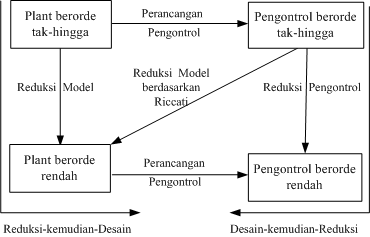
\includegraphics[scale=0.7]{assets/pict/reduksi_design.png}\\
\caption{Alternatif perancangan pengontrol berorde rendah}\label{desain}
\end{figure}
Berikut pemisalan untuk menulis endnote \cite{CZ95}.
\section{Rumusan Masalah}

Rumusan masalah merupakan bagian terpenting dari bab pendahuluan yang umumnya dibaca terlebih dahulu oleh pembaca skripsi. Melalui rumusan masalah dapat secarasingkat diketahui hal yang akan diteliti dalam skripsi. Rumusan masalah berupa pertanyaan-pertanyaan yang ingin dicari jawabannya melalui kegiatan ilmiah yang akan dilakukan. Rumusan masalah terkait integrasi keagamaan dapat dicantumkan jika diperlukan dengan tetap mendahulukan rumusan masalah terkait keilmuan \cite{Curtain03}.
\section{Tujuan Penelitian}

Tujuan penelitian harus menyebutkan secara khusus hal yang ingin dicapai. Dalam beberapa hal, tujuan penelitian sudah tersirat di dalam judul penelitian dan latar belakang. Tujuan penelitian harus sesuai dengan rumusan masalah yang diajukan.
\section{Manfaat Penelitian}

Manfaat penelitian terutama ditujukan bagi pengembangan ilmu atau pelaksanaan pembangunan dalam arti luas. Dengan kata lain, manfaat penelitian berisi alasan kelayakan atas masalah yang diteliti.Dari uraian dalam bagian ini, diharapkan dapat disimpulkan bahwa penelitian terhadap masalah yang dipilih memanglayak untuk dilakukan. Manfaat penelitian perlu dibedakan segi kepentingannya, misalnya segi teoritis atau praktis dan segi tujuannya, misalnya bagi penulis, lembaga, atau pihak-pihak lain.
\section{Batasan Masalah}

Batasan masalah dibuat jika penelitian memerlukan batasan-batasan tertentu untuk menjelaskan ruang lingkup penelitian. Batasan masalah ini juga diperlukan untuk lebih mengarahkan atau memfokuskan penelitian. Batasan masalah tidak berisi masalah dalam rumusan masalah, tetapi batasan-batasan yang diperlukan untuk membatasi masalah.
\section{Metode Penelitian}

Metode penelitian untuk penelitian kepustakaan (library research) dapat ditempatkan di bagian pendahuluan. Dalam bagian ini, dijelaskan metode penelitian yang diambil disertai alasan mengapa metode tersebut dipilih untuk menjawab masalah. Dalam metode penelitian juga dijelaskan tahap-tahap atau langkah-langkah rinci penelitian untuk sampai pada tujuan yang ingin dicapai. Pada Penelitian kepustakaan Metode Penelitian ditempatkan pada BAB I.

Metode penelitian untuk penelitian aplikasi atau studi kasus memuat uraian tentang jenis penelitian, data dan sumber data, alat pengumpul data, metode pengumpulan data, tahap-tahap penelitian,dan analisis hasil penelitian. Penjelasan dalam metode penelitian dapat dilengkapi dengan diagram alur yang berfungsi untuk memperjelas uraian. Pada Penelitian aplikasi Metode Penelitian ditempatkan pada BAB III.
\section{Sistematika Penulisan}

Sistematika penulisan bukanlah pemindahan daftar isi. Sistematika penulisan diberikan untuk menyajikansecara naratif outline penulisan bagian utama skripsi, yang meliputi susunanbab dan topik-topik pokok yang ada dalam bab.